\chapter{Implementazione del Framework}
In questo capitolo viene esposto l'intero framework di compressione proposto, costruito sulle fondamenta teoriche esposte nel Capitolo \ref{cap:teoria}.

\section{Gestione e Divisione dei dati}
Nella fase iniziale il framework di compressione prevede di istanziare il dataset. In particolare, inizialmente viene eseguita la suddivisione in \textit{Dati di Train} e \textit{Dati di Test}, successivamente i primi vengono ulteriormente divisi in \textit{Training Set} e \textit{Validation Set}. Il secondo di questi verrà utilizzato esclusivamente per monitorare l'accuratezza del modello durante le iterazioni di compressione. Per quanto concerne il \textit{Training Set}, questo viene utilizzato alla fine di ogni iterazione per eseguire una serie di epoche di \textit{Fine Tuning}, al fine di permettere un riadattamento dei parametri del modello, ma anche come sorgente da cui estrarre il \textit{Search Set}. \par
Quest'ultimo è formato da un numero ben preciso di campioni per classe $N$, che costituisce un iper-parametro del processo di compressione, in questo modo la sua dimensione corrisponde ad $N \times |Classes|$. Dagli esperimenti effettuati emerge un valore ottimale di $N$ di 25 campioni per classe, poiché permette una buona approssimazione dei gradienti, ma allo stesso tempo consente di mantenere contenuto il tempo necessario alla fase di ricerca. Infatti, il \textit{Search Set} viene utilizzato su ogni nodo dell'albero di ricerca (ovvero su ogni \textit{Subnet}) sia per il calcolo della metrica di importanza per ogni parametro (che prevede quindi un passo di \textit{backpropagation}, dal grande costo computazionale), sia per la valutazione dell'accuratezza.
\begin{figure}[H]
    \centering
    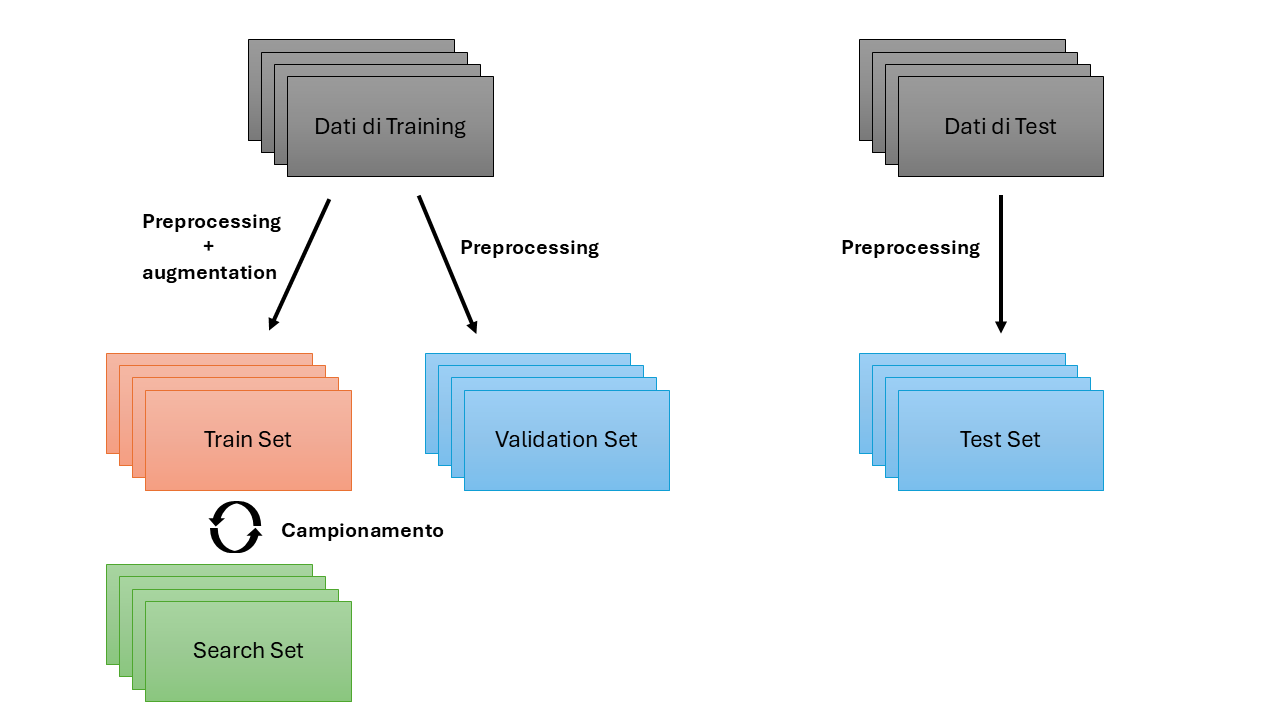
\includegraphics[width=0.7\textwidth]{images/split_dataset.png}
    \caption{Processo di suddivisione del dataset adottato.}
\end{figure}
Per evitare che la fase di ricerca, utilizzando un unico \textit{Search Set} per tutte le iterazioni, provochi un \textit{\textbf{Overfitting Architetturale}}, con conseguenti difficoltà di generalizzazione del modello compresso, il \textit{Search Set} viene \textbf{campionato ad ogni iterazione} a partire dal \textit{Training Set}, fornendo campioni differenti all'algoritmo, di iterazione in iterazione. Questo permette di ottenere un modello risultante che è in grado di generalizzare al meglio sul problema di classificazione, proprio perché l'architettura finale, è il risultato ottenuto con una maggiore quantità e varietà di dati. \par
Un altro contributo fondamentale al mantenimento della capacità di generalizzazione del modello, è dato dalla \textbf{Data Augmentation}, che viene sempre applicata al \textit{Search Set}, ed è la stessa che viene applicata ai dati del \textit{Training Set}. Si potrebbe pensare che questo introduca rumore nei gradienti, e quindi influenzi la precisione e l'affidabilità della metrica di importanza. Nella pratica però il problema del rumore è fortemente limitato dall'utilizzo della media dei gradienti sui batch, per il calcolo della metrica di importanza, com'è possibile osservare nella Formula~\eqref{eq:metrica_importanza}. La \textit{Data Augmentation} applicata al \textit{Search Set} è risultata molto efficace, nei test effettuati, per impedire che venissero sacrificate delle dimensioni del modello essenziali per mantenere la sua capacità di generalizzazione, traducendosi in questo modo in valori di accuratezza sul \textit{Test Set} e sul \textit{Validation Set} più elevati durante tutta l'esecuzione del framework. \par
Notare che è possibile interpretare il framework di compressione come un \textbf{ottimizzazione a due livelli} del modello. In particolare il livello superiore è occupato dal processo di ricerca, che esegue un vero e proprio \textbf{training architetturale}, mentre il livello inferiore è quello del \textit{Fine Tuning}, che invece si occupa di \textbf{ottimizzare i parametri}, date le modifiche architetturali operate dal livello superiore. Questa visione del metodo permette di comprendere al meglio le motivazioni dietro la specifica gestione dei dati, ed in particolare del \textit{Search Set}. Infatti, l'applicazione di tecniche di \textit{data augmentation} a quest'ultimo implica una dinamicità che contribuisce a scongiurare il fenomeno dell'\textit{overfitting architetturale}, analogamente a come tecniche quali l'\textit{early stopping} o i \textit{Learning Rate Scheduler} vengono impiegate per prevenire l'\textit{overfitting} dei parametri del modello.

\section{Framework di Compressione Iterativo}
Una volta definita la strategia di gestione dei dati, è necessario definire la struttura del framework di compressione iterativo, in particolare cosa avviene ad ogni iterazione. \par
\begin{figure}[H]
    \centering
    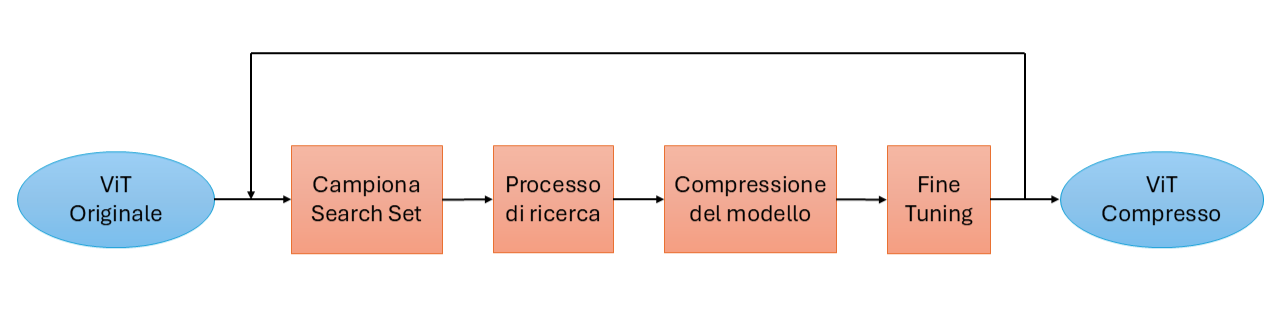
\includegraphics[width=0.9\textwidth]{images/processo.png}
    \caption{Diagramma di flusso del processo di compressione iterativo.}
    \label{fig:processo_compressione}
\end{figure}
Inizialmente viene campionato il \textit{Search Set}, in modo tale da poterlo utilizzare in fase di ricerca. Successivamente inizia la prima fase dell'iterazione: il \textbf{Pruning}. La prima operazione che viene eseguita è l'algoritmo di ricerca \textit{BnB}, che verrà analizzato nella sezione \ref{section:metodo_ricerca}, il quale restituisce lo stato migliore individuato, ovvero una maschera di \textit{pruning} per l'intero modello. \par
A questo punto la maschera viene applicata al modello, e questo viene successivamente ricostruito istanziando tutti i tensori dei parametri ed effettuando una copia solo di quelli non tagliati in fase di ricerca. Viene quindi creato un nuovo modello \textit{ViT}, del quale sono state effettivamente ridotte le dimensioni e questo risulta fondamentale perché implica che il framework proposto non si limita ad applicare delle maschere di \textit{pruning}, che non avrebbero alcun impatto sulle prestazioni effettive del modello sull'hardware, bensì produce dei nuovi modelli di dimensioni realmente minori, con prestazioni realmente superiori. In particolare viene ridotta la latenza in fase di inferenza ma anche la memoria necessaria (VRAM) per utilizzare il modello. \par
Una volta ricostruito il modello, dato che la fase di \textit{Pruning}, avrà introdotto un danno alle performance del modello, è necessario passare alla successiva fase di \textbf{Recovery Fine Tuning}. Si tratta di una serie di epoche di addestramento, volte a consentire ai parametri rimasti del modello di riadattarsi, per poter recuperare l'accuratezza perduta. Risulta fondamentale in questa fase la possibilità di introdurre la \textit{Knowledge Distillation} tramite il modello originale non compresso, che permette tipicamente un recupero più efficace della performance del modello. \par
\begin{algorithm}[H]
\caption{Framework di Compressione Iterativo}
\label{alg:framework_completo}
\begin{algorithmic}[1]
    \State \textbf{Input:} Pre-trained model $M_0$, Dataset $\mathcal{D}$, Iterations $N$, Fine Tuning epochs $K$
    \State \textbf{Output:} Compressed and optimized model $M$
    \State $M_{teacher} \gets M_0$ \Comment{Original model used for distillation}
    \State $M \gets M_0$
    
    \For{$n \gets 1$ \textbf{to} $N$}
        \State $\mathcal{D}_{search} \gets \text{sample\_search\_set}(\mathcal{D}_{train})$ \Comment{Dynamic sampling of the search set}
        \State $m_{pruning} \gets \text{pruning\_algorithm}(M, \mathcal{D}_{search})$ \Comment{obtain pruning mask}
        \State $M_{pruned} \gets \text{compress\_ViT}(M, m_{pruning})$ \Comment{Rebuilding ViT}
        \State $M \gets M_{pruned}$ 
        \State $M \gets \text{FineTuning}(M, M_{teacher}, \mathcal{D}_{train}, \mathcal{D}_{val}, K)$
    \EndFor
    
    \State \Return $M$
\end{algorithmic}
\end{algorithm}

\section{Implementazione dell'algoritmo di ricerca}
\label{section:metodo_ricerca}
In questa sezione viene dettagliata l'implementazione della fase di ricerca con algoritmo \textit{Branch and Bound}, che viene eseguito all'inizio di ogni iterazione di compressione. \par
Al fine di evitare una eccessivo utilizzo di memoria, il processo di ricerca fa utilizzo di stati costituiti come strutture dati a dizionario, invece che vere e proprie copie del modello originale. All'interno di ogni stato è presente una struttura che, per ogni blocco \textit{Transformer} contiene tutte le dimensioni rimosse per ogni tipologia di struttura (MLP, QK, ecc\dots), oltre ad una informazione generale su quali dimensioni di \textit{Embedding} sono state tagliate globalmente. \par
A partire da questa struttura dati è possibile agire su una serie di maschere di \textit{pruning} che vengono applicate al modello, permettendo così di ottenere la vera e propria \textit{subnet}. Per garantire la massima efficienza queste maschere vengono applicate ad un'unica copia del modello iniziale, che, alla fine di ogni esplorazione dello stato vede le proprie maschere reimpostate, per poter applicare i tagli previsti dal successivo stato della ricerca.
\begin{algorithm}[H]
\caption{Ricerca via Depth-First Branch and Bound a profondità limitata}
\label{alg:nas_search}
\begin{algorithmic}[1]
    \State \textbf{Input:} Base Model $M$, Depth Limit $D_{max}$
    \State \textbf{Output:} Optimal State $s_{best}$, Optimal State value $v_{best}$
    \State $s_{init} \gets \text{build\_initial\_state}()$
    \State $stack \gets [s_{init}]$ \Comment{Stack setup}
    \State $M_{work} \gets \text{copy}(M)$
    \State $s_{best} \gets s_{init}$
    \State $v_{best} \gets -\infty$
    \While{$stack$ is not empty}
        \State $s_{curr} \gets stack.\text{pop}()$
        \State $\text{reset\_masks}(M_{work})$
        \State $\text{apply\_masks}(M_{work}, s_{curr})$
        \State $accuracy, active\_params \gets \text{evaluate}(M_{work})$ \Comment{Subnet evaluation}
        \State $v_{curr} \gets \text{compute\_obj}(acc, active\_params)$

        \If{$v_{curr} > v_{best}$}
            \State $v_{best}, s_{best} \gets v_{curr}, s_{curr}$
        \EndIf
        \If{$D_{max}$ reached \textbf{OR} $\text{Bound}(v_{curr}, v_{best})$}
            \State \textbf{continue} \Comment{Bound or depth limit reached}
        \EndIf
        \State // \textit{Branching}
        \State $next\_states \gets \text{Branch}(s_{curr}, M_{work})$
        \For{$s$ in $next\_states$}
            \State $stack.\text{push}(s)$
        \EndFor
    \EndWhile
    
    \State \Return $s_{best}, v_{best}$
\end{algorithmic}
\end{algorithm}




\section{Implementazione delle azioni di Pruning}
\label{section:action_impl}
Data la formulazione matematica delle azioni di ricerca, presentata nella sezione \ref{section:math_actions}, in fase di implementazione, considerato l'elevatissimo numero di dimensioni nel modello, viene addottato un approccio più efficiente.
In particolare, non vengono considerate realmente tutte le possibili combinazioni di dimensioni a $K$ a $K$ di un componente del modello, poiché, dato che è di interesse la somma delle importanze delle singole dimensioni, è sufficiente considerare le $K$ dimensioni le cui importanze sono minime. In particolare, per tutte quelle azioni che agiscono all'interno di un singolo blocco (ovvero tutte tranne il \textit{Pruning} della dimensione di \textit{Embedding}), vengono identificate, per ogni blocco \textit{Transformer} le $K$ dimensioni con il minor valore di importanza. Successivamente, viene selezionato il blocco, il cui gruppo di dimensioni ottimali, hanno una importanza complessiva minore. Questo tipo di approccio semplifica e rende la risoluzione del problema più efficiente. \par
Per quanto riguarda il \textit{Pruning} della dimensione di \textit{Embedding}, l'approccio adottato è il medesimo, con la differenza che, essendo questa una dimensione globale, non vengono considerati singolarmente i blocchi ma complessivamente, riducendo l'algoritmo all'individuazione dei $K$ minimi valori di importanza sull'intero modello. \par
\begin{algorithm}[H]
\caption{Selezione del gruppo di dimensioni ottimale per il taglio}
\label{alg:find_target_gen}
\begin{algorithmic}[1]
    \State \textbf{Input:} Model $M$, Chunk size $K$, Target component $T$
    \State \textbf{Output:} $(\text{block}, [\text{dimension indices}])$ Target dimension group
    \State $v_{best\_imp} \gets \infty$
    \State $target \gets \text{null}$
    
    \For{every block $b$ in $M.blocks$}
        \If{number of dimensions in $T(b) < K$}
            \State \textbf{continue}
        \EndIf
        
        \State $candidates \gets \emptyset$
        
        \For{every dimension $d$ in $T(b)$}
            \If{$d$ is already pruned}
                \State \textbf{continue}
            \EndIf
            \State $imp_d \gets \text{importance\_score}(d)$
            \State $candidates.\text{append}((d, imp_d))$
        \EndFor
        
        \State $candidates \gets$ sort($candidates$, ascending = True) 
        \State $chunk \gets candidates[0 : K]$
        \State $v_{block\_imp} \gets \sum_{(d, i) \in chunk} i$
        
        \If{$v_{block\_imp} < v_{best\_imp}$}
            \State $v_{best\_imp} \gets v_{local\_imp}$
            \State $target \gets (b, \text{chunk.indices})$
        \EndIf
    \EndFor
    
    \State \Return $target$
\end{algorithmic}
\end{algorithm}
